%\subsection{Aplicativo}

	\par O primeiro passo realizado para a construção do aplicativo Android, foi a
modelagem do software através dos diagramas de UML, que permitiram nortear o
desenvolvimento.

	\par A princípio projetou-se um diagrama para se ter uma visão geral do
aplicativo. Nele pode-se ver a arquitetura da aplicação, bem como a comunicação
com o GCM e o \textit{web service}.

	\par Quando o servidor precisa enviar uma informação para os dispositivos
móveis, ele envia a mensagem ao GCM, que a transfere para aplicativo. Ao
receber os dados, a classe \texttt{GcmBroadcastReceiverUnivas} executa a classe
\texttt{GcmIntentServiceUnivas} que por sua vez irá notificar o usuário,
contudo antes de notificá-lo, ela envia as informações para a classe
\texttt{HttpUtil}, que faz a conversão dos dados vindos em JSON para o formato
da classe \texttt{EventTO}. Ao finalizar a leitura e conversão dos elementos,
as informações são enviadas para a classe \texttt{DatabaseExecute} que realiza
a gravação dos dados no banco de dados.

	\par Quando o usuário clica na notificação, é apresentada a ele uma
\textit{activity} a qual exibe as informações recebidas. Neste contexto, quando
se tratar de uma nota será aberta a \textit{activity}
\texttt{NotificationResultsActivity}, no caso de ser uma falta é executada a
\textit{activity} \texttt{NotificationFoulsActivity} e caso for um evento de
provas agendadas então é mostrada a \textit{activity}
\texttt{NotificationAgendasActivity}.

	\par Para o estudante visualizar suas informações, ele acessará a classe
\texttt{MainActivity}. Se desejar ver as suas notas, então é apresentada a
\textit{activity} \texttt{ListResultsActivity}, que utiliza a classe
\texttt{ListResultsAdapter} para gerenciar as informações e apresentá-las ao
discente. No entanto, se escolher a opção de faltas, é apresentada a
\textit{activity} \texttt{ListFoulsActivity}, que receberá as informações da
classe \texttt{ListFoulsAdapter} e caso decida-se pela opção provas agendadas é
exibida a \textit{activity} \texttt{ListAgendasActivity}, gerenciada pela
classe \texttt{ListAgendasAdapter}.

	\par A classe \texttt{GcmControllerUnivas}, tem por finalidade cadastrar o
dispositivo no GCM e enviar a chave gerada para o \textit{web service}. Na
Figura \ref{fig:app}, é apresentado o diagrama de arquitetura.

	\begin{figure}[h!] 
		\centerline{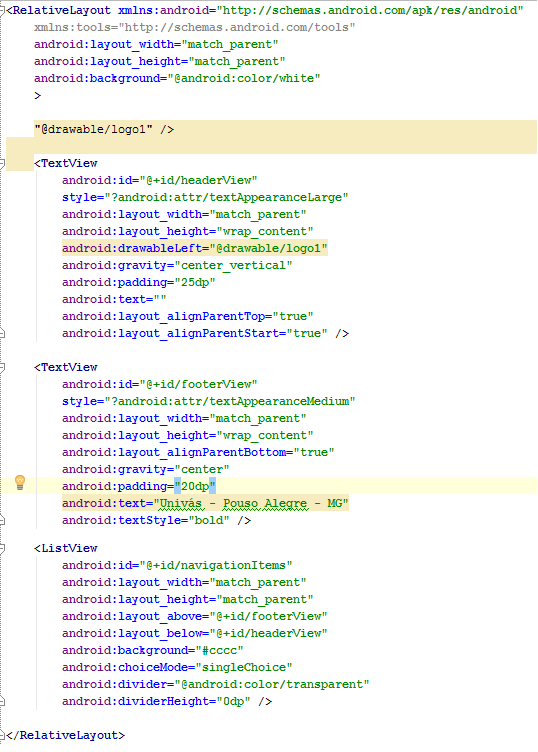
\includegraphics[scale=0.42]{./imagens/2_q_metodologico/4_procedimentos_resultados/42_aplicativo/app.png}}
		\caption[Diagrama de arquitetura do aplicativo]{Diagrama de arquitetura do aplicativo.
		\textbf{Fonte:}Elaborado pelos autores.}
		\label{fig:app}
	\end{figure}
	
	\par Posteriormente, foi desenvolvido o diagrama de caso de usos, com
finalidade em ter uma visão das funcionalidades do software pelo lado do
usuário. O utilitário permite ao aluno receber notificações quando for lançada
uma nova nota, falta ou prova agendada e visualizar estas informações. Na
Figura \ref{fig:app1} é possível ver o diagrama de casos de uso.

	\begin{figure}[h!] 
		\centerline{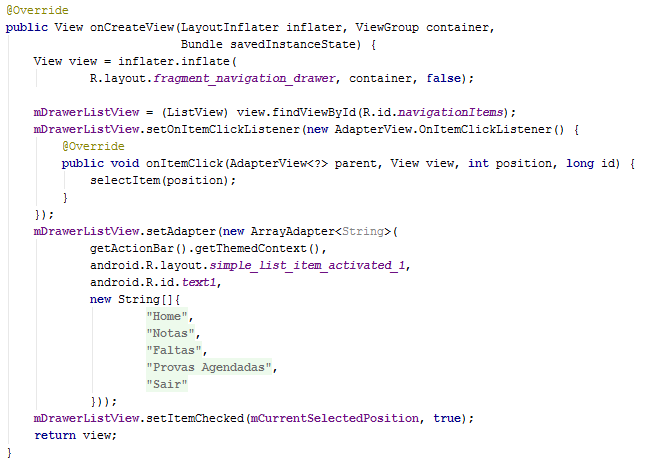
\includegraphics[scale=0.7]{./imagens/2_q_metodologico/4_procedimentos_resultados/42_aplicativo/app1.png}}
		\caption[Diagrama de casos de uso]{Diagrama de casos de uso.
		\textbf{Fonte:}Elaborado pelos autores.}
		\label{fig:app1}
	\end{figure}
	
	\par Para iniciar a construção do aplicativo, fez-se necessário a instalação e
configuração do ambiente de desenvolvimento. Primeiramente, realizou-se o
\textit{download} da IDE Android Studio, versão 1.1.0 e do Android SDK, versão
24.0.2, ambos no site \textit{Developers} Android através do endereço
\url{https://developer.android.com/intl/pt-br/sdk/index.html}.

	\par Contudo, ao executar o emulador do Android o sistema apresentava a
seguinte mensagem: “\textit{emulator: Failed to open the HAX device!}”. Depois
de algum tempo pesquisando, percebeu-se que era necessário instalar um programa
chamado Intel \textit{Hardware Accelerated Execution Manager} (HAXM), que
permite a execução do emulador Android mais rápido.

	\par No entanto, ao instalá-lo ocorria o seguinte erro: “\textit{this computer
meets the requirements for haxm but intel virtualization technology (VT-x) is
not turned on.}” A solução foi acessar a BIOS da máquina e habilitar o
assistente de hardware para virtualização. Daí em diante, foi possível executar
no emulador as aplicações feitas no Android Studio.

	\par Com o ambiente já configurado, foi criado um repositório no controlador de
versão Github, o qual pode ser acessado através do endereço
\url{https://github.com/diegodnunes12/AppTCC} e compartilhado entre os
participantes do projeto.

	\par A partir de então, passou-se a desenvolver o software. A princípio, foi
construída uma \textit{activity}, que é acessível ao aluno logo que a aplicação
se inicia. Essa \textit{activity} é do tipo \textit{Navigation Drawer Layout},
ou seja, é um painel que permite inserir as opções de navegação do aplicativo,
semelhante a um menu.

	\par Ao criar essa \textit{activity}, o Android Studio gera automaticamente a
classe \texttt{NavigationDrawerFragment} e um arquivo XML na pasta
\textit{layout}, chamado \texttt{fragment\_navigation\_drawer.xml}.

	\par No arquivo \texttt{fragment\_navigation\_drawer.xml} foram inseridos três
\textit{widgets}, sendo dois do tipo \texttt{textView}, para o cabeçalho com a
logomarca da Univás e para o rodapé com o seguinte texto: “Univás – Pouso
Alegre – MG” e um \textit{widget} do tipo \texttt{listView} que contém a lista
com as opções que o software oferece ao aluno.

	\par O \textit{layout} desta \textit{activity} chama-se
\textit{relativeLayout}, o qual permite um elemento ser posicionado em relação
ao outro. Desta forma o \textit{widget} \textit{listView} utiliza a propriedade
\texttt{android:layout\_below="@+id/headerView"} para se posicionar abaixo do
componente com id \textit{headerView} e a propriedade
\texttt{android:layout\_above="@+id/footerView"} indicando que ela deve preceder
o \textit{widget} com id \textit{footerView}. Na Figura \ref{fig:app2}, pode
ser visto o código XML dos \textit{widgets} desta tela.

	\begin{figure}[h!] 
		\begin{lstlisting}[style=custom_XML]
	<RelativeLayout xmlns:android="http://schemas.android.com/apk/res/android"
    xmlns:tools="http://schemas.android.com/tools"
    android:layout_width="match_parent"
    android:layout_height="match_parent"
    android:background="@android:color/white">
	    <TextView
	        android:id="@+id/headerView"
	        style="?android:attr/textAppearanceLarge"
	        android:layout_width="match_parent"
	        android:layout_height="wrap_content"
	        android:drawableLeft="@drawable/logo1"
	        android:gravity="center_vertical"
	        android:paddingTop="5dp"
	        android:paddingBottom="5dp"
	        android:paddingLeft="25dp"
	        android:paddingRight="25dp"
	        android:text=""
	        android:layout_alignParentTop="true"
	        android:layout_alignParentStart="true" />
	    <TextView
	        android:id="@+id/footerView"
	        style="?android:attr/textAppearanceMedium"
	        android:layout_width="match_parent"
	        android:layout_height="wrap_content"
	        android:layout_alignParentBottom="true"
	        android:gravity="center"
	        android:padding="20dp"
	        android:textColor="#228B22"
	        android:text="Univas - Pouso Alegre - MG"
	        android:textStyle="bold" />
	    <ListView
	        android:id="@+id/navigationItems"
	        android:layout_width="match_parent"
	        android:layout_height="match_parent"
	        android:layout_above="@+id/footerView"
	        android:layout_below="@+id/headerView"
	        android:background="#228B22"
	        android:choiceMode="singleChoice"
	        android:divider="@android:color/transparent"
	        android:dividerHeight="1dp" />
</RelativeLayout>
\end{lstlisting}
		\caption[Código dos widgets do arquivo
		fragment\_navigation\_drawer.xml]{Código dos \textit{widgets} do arquivo
		\texttt{fragment\_navigation\_drawer.xml}.
		\textbf{Fonte:}Elaborado pelos autores.}
		\label{fig:app2}
	\end{figure}
	
	\pagebreak
	
	\par A classe \texttt{NavigationDrawerFragment} representa o painel de
navegação. Nela se destaca o método \texttt{onCreateView()}, responsável por
criar o \textit{layout} de navegação. Na Figura \ref{fig:app3}, é mostrado o
método \texttt{onCreateView()} informando ao sistema operacional o \textit{layout} a
ser carregado e adicionando a um \textit{array} de \textit{String} as
alternativas de navegação que serão exibidos no \textit{listView} da tela
principal. Pode-se perceber também o método \texttt{onItemClick()}, que é
executado no momento em que o usuário clica em algum item da lista. 
	


	\begin{figure}[h!] 
		\begin{lstlisting}[style=custom_JAVA]
@Override
public View onCreateView(
		LayoutInflater inflater, ViewGroup container,Bundle savedInstanceState) {
    View view = inflater.inflate(
            R.layout.fragment_navigation_drawer, container, false);

    mDrawerListView = (ListView) view.findViewById(R.id.navigationItems);
    mDrawerListView.setOnItemClickListener(new AdapterView.OnItemClickListener() {
        @Override
        public void onItemClick(AdapterView<?> parent, View view, int position, long id) {
            selectItem(position);
        }
    });
    mDrawerListView.setAdapter(new ArrayAdapter<String>(
            getActionBar().getThemedContext(),
            android.R.layout.simple_list_item_activated_1,
            android.R.id.text1,
            new String[]{
                    getString(R.string.title_section1),
                    getString(R.string.title_section2),
                    getString(R.string.title_section3),
                    getString(R.string.title_section4),
                    getString(R.string.title_section5)
            }));
    mDrawerListView.setItemChecked(mCurrentSelectedPosition, true);
    return view;
}
public boolean isDrawerOpen() {
    return mDrawerLayout != null && mDrawerLayout.isDrawerOpen(mFragmentContainerView);
}
\end{lstlisting}
		\caption[Método onCreateView()]{Método \texttt{onCreateView()}.
		\textbf{Fonte:}Elaborado pelos autores.}
		\label{fig:app3}
	\end{figure}
	
	\pagebreak
	
	\par Nesse caso, quando for selecionada alguma opção da tela principal será
executado o método \texttt{selectItem()} apresentado na Figura \ref{fig:app4}, o
qual é responsável por retornar a posição do \textit{array} em que se encontra a
opção selecionada pelo aluno.
	
	\begin{figure}[h!] 
		\begin{lstlisting}[style=custom_JAVA]
	private void selectItem(int position) {
        mCurrentSelectedPosition = position;
        if (mDrawerListView != null) {
            mDrawerListView.setItemChecked(position, true);
        }
        if (mDrawerLayout != null) {
            mDrawerLayout.closeDrawer(mFragmentContainerView);
        }
        if (mCallbacks != null) {
            mCallbacks.onNavigationDrawerItemSelected(position);
        }
    }
\end{lstlisting}
		\caption[método selectItem()]{método \texttt{selectItem()}.
		\textbf{Fonte:}Elaborado pelos autores.}
		\label{fig:app4}
	\end{figure}
	
	\par O próximo passo foi criar o banco de dados do aplicativo para salvar as
informações recebidas do \textit{web service}. Para que isso fosse possível,
elaborou-se uma classe denominada \texttt{DatabaseHelper} que estende da classe
\texttt{SQLiteOpenHelper} do Android, com dois métodos, um chamado
\textit{onCreate()} que cria a estrutura do banco de dados e outro conhecido
por \textit{onUpgrade()}, usado se for necessário atualizar a estrutura do
banco de dados.

	\par Foi preciso criar um atributo que mantém a versão do banco de dados. Essa
informação serve para que o Android consiga saber qual dos dois métodos devem
ser executados. Ao iniciar a aplicação pela primeira vez, estando a versão em 1
(um), o sistema chamará o método \texttt{onCreate()}. Se for preciso atualizar
a estrutura do banco, o atributo versão deve ser incrementado em 1 (um), de
modo que ao executar o software o sistema operacional perceba a mudança,
chamando o método \texttt{onUpgrade()}. Na Figura \ref{fig:app5} é apresentado a
classe \texttt{DatabaseHelper}.

	\begin{figure}[h!] 
		\begin{lstlisting}[style=custom_JAVA]
public class DatabaseHelper extends SQLiteOpenHelper {

    private static final String BANCO_DADOS = "univasDB";
    private static int VERSAO = 1;

    public DatabaseHelper(Context context) {
        super(context, BANCO_DADOS, null, VERSAO);
    }
    @Override
    public void onCreate(SQLiteDatabase db) {
        db.execSQL("CREATE TABLE disciplinas (_id LONG PRIMARY KEY, nome TEXT);");

        db.execSQL("CREATE TABLE eventos (_id LONG PRIMARY KEY, id_disciplina LONG, " +
                " tipo_evento TEXT, descricao_evento TEXT," +
                " data_evento TEXT, valor_evento INTEGER, nota INTEGER,"  +
                " FOREIGN KEY (id_disciplina) REFERENCES disciplinas (_id) );");
    }
    @Override
    public void onUpgrade(SQLiteDatabase db, int i, int i2) {
        //Nao ha atuaizacoes no momento
    }
}
\end{lstlisting}
		\caption[Classe DatabaseHelper]{Classe \texttt{DatabaseHelper}.
		\textbf{Fonte:}Elaborado pelos autores.}
		\label{fig:app5}
	\end{figure}
	
	\par Em seguida foi criada a classe responsável por executar as consultas SQL,
denominada \texttt{DatabaseExecute}. Nela foram inseridos os métodos
responsáveis por inserir, alterar e buscar os dados dos alunos no banco de
dados local do aplicativo. Na Figura \ref{fig:app6}, pode-se observar o método
que possibilita a inserção dos eventos ocorridos. Esses eventos podem ser
notas, faltas ou provas agendadas.
	
	
	\begin{figure}[h!] 
		\begin{lstlisting}[style=custom_JAVA]
public void insertEvents(EventTO to){
        SQLiteDatabase db = helper.getWritableDatabase();

        ContentValues values = new ContentValues();
        values.put("_id", to.get_id());
        values.put("id_disciplina", to.getId_discipline());
        values.put("tipo_evento", to.getType_event());
        values.put("descricao_evento", to.getDescription_event());
        values.put("data_evento", to.getDate_event());
        values.put("valor_evento", to.getValue_event());
        values.put("nota", to.getResult());

        long result = db.insert("eventos", null, values);

        if(result != -1 ){
            Log.d(TAG, " Evento salvo com sucesso!");
        }else{
            Log.d(TAG, " Erro ao salvar o Evento!");
        }
    }
\end{lstlisting}
		\caption[Método de inserção de eventos]{Método de inserção de eventos.
		\textbf{Fonte:}Elaborado pelos autores.}
		\label{fig:app6}
	\end{figure}
	
	\pagebreak
	
	\par Este método recebe um objeto da classe \texttt{EventTO} com os elementos
necessários para inserir o evento no banco de dados. Para que seja possível a
inserção dos dados, \citeonline{monteiro2012}, afirma que é necessário
recuperar a referência da classe \texttt{SQLiteDatabase} através do método
\texttt{getWritableDatabase()}, logo após é instanciada a classe
\texttt{ContentValues}, onde são informados os campos da tabela e os
respectivos valores. Ao concluir, é chamado o \texttt{insert()} da classe
\texttt{SQLiteDatabase} informando o nome da tabela e o objeto da classe
\texttt{ContentValues}.

	\par Para listar os resultados dos exames realizados pelos discentes no painel
de notas é utilizado o método \texttt{getResults()} que retorna uma lista de
objetos da classe \texttt{EventTO}. De acordo com \citeonline{monteiro2012},
para conseguir recuperar as informações armazenadas no banco de dados é preciso
adquirir a instância de leitura da classe \texttt{SQLiteDatabase} através do
método \texttt{getReadableDatabase()}. Por meio dele pode-se realizar a
consulta, que devolve um \textit{Cursor} para navegar pelos resultados. Por
fim, é composto um objeto do tipo \texttt{EventTO} e inserido na lista. Na
Figura \ref{fig:app7} é apresentado o método \texttt{getResults()}.

	\par Foram inseridos mais dois métodos semelhantes ao \texttt{getResults()},
que são os métodos de \texttt{getFouls()} e \texttt{getAgendas()} para
recuperar as faltas e provas agendadas respectivamente. O que diferencia-os é a
consulta SQL, já que no \texttt{getFouls()}  foram buscados os dados onde o
\texttt{tipo\_evento = ‘FALTAS'} e no \texttt{getAgendas()} onde o
\texttt{tipo\_evento = ‘PROVA\_AGENDADA'}.

	\begin{figure}[h!] 
		\begin{lstlisting}[style=custom_JAVA]
public List<EventTO> getResults(){
        List<EventTO> notasTO = new ArrayList<>();

        SQLiteDatabase db = helper.getReadableDatabase();
        Cursor cursor =
                db.rawQuery("SELECT _id, id_disciplina, descricao_evento, valor_evento, nota  FROM" +
                                " eventos WHERE tipo_evento = 'PROVA_APLICADA'",
                        null);
        cursor.moveToFirst();

        for(int i = 0; i<cursor.getCount();i++){
            EventTO nota = new EventTO();

            nota.set_id(cursor.getLong(0));
            nota.setId_discipline(cursor.getLong(1));
            nota.setDescription_event(cursor.getString(2));
            nota.setValue_event(cursor.getInt(3));
            nota.setResult(cursor.getInt(4));

            notasTO.add(nota);
            cursor.moveToNext();
        }
        cursor.close();
        return notasTO;
    }
\end{lstlisting}
		\caption[Método getResults()]{Método \texttt{getResults()}.
		\textbf{Fonte:}Elaborado pelos autores.}
		\label{fig:app7}
	\end{figure}
	
	\pagebreak
	
	\par A fim de estabelecer uma conexão entre o aplicativo e o \textit{web
service}, foi preciso conceder a permissão de acesso à internet no arquivo
\texttt{AndroidManifest.xml} da seguinte forma: \texttt{<uses-permission
android:name="android.permission.INTERNET" />}.

	\par Logo após, criou-se uma classe chamada de \texttt{HttpUtilUnivas} para ler
informações recebidas do \textit{web service}. Ela estende da classe
\texttt{AsyncTask} que executa a consulta em paralelo com a \textit{thread
main}, evitando travar a aplicação enquanto recebe as informações vindas do
\textit{web service}. Estes dados estão em formato JSON e foi utilizada a
biblioteca GSON para convertê-las para o formato da classe \texttt{EventTO}.
Após a leitura, o objeto da classe \texttt{EventTO} é enviado para a classe
\texttt{DatabaseExecute}, a fim de realizar a inserção os dados no banco. A
Figura \ref{fig:app8}, mostra a classe \texttt{HttpUtilUnivas}.

	\begin{figure}[h!] 
		\begin{lstlisting}[style=custom_JAVA]
try{
        HttpClient httpClient = new DefaultHttpClient();
        HttpGet request = new HttpGet();
        request.setURI(new URI(urlEvents));

        HttpResponse response = null;
        try {
            response = httpClient.execute(request);
        } catch (IOException e) {
            e.printStackTrace();
        }
        InputStream content = null;
        try {
            content = response.getEntity().getContent();
        } catch (IOException e) {
            e.printStackTrace();
        }
        Reader reader = new InputStreamReader(content);
        Gson gson = new Gson();
        returnEvents = gson.fromJson(reader, Events.class);

        for (int i = 0; i< returnEvents.getEventos().size(); i++){
            DatabaseExecute execute = new DatabaseExecute(helper);
            EventTO to = new EventTO();
            to.set_id((long) returnEvents.getEventos().get(i).getId_evento());
            to.setValue_event(returnEvents.getEventos().get(i).getValor());
            to.setDescription_event(returnEvents.getEventos().get(i).getDescricao());
            to.setId_discipline(returnEvents.getEventos().get(i).getId_disciplina());
            to.setDate_event(returnEvents.getEventos().get(i).getData());
            to.setResult(returnEvents.getEventos().get(i).getNota());
            to.setType_event(returnEvents.getEventos().get(i).getTipoEvento());

            if(execute.existingEvent(to.get_id()) == false){
                execute.insertEvents(to);
            }else{
                execute.updateEvent(to);
            }
        }
        content.close();
    } catch (URISyntaxException e) {
        e.printStackTrace();
    } catch (IOException e) {
        e.printStackTrace();
    }
\end{lstlisting}
		\caption[Código da classe HttpUtilUnivas que faz a leitura dos
		eventos]{Código da classe \texttt{HttpUtilUnivas} que faz a leitura dos
		eventos.
		\textbf{Fonte:}Elaborado pelos autores.}
		\label{fig:app8}
	\end{figure}
	
	\pagebreak
	
	\par Para usufruir da biblioteca GSON, foi fundamental adicioná-la como uma
dependência do projeto. Para isso, foi preciso ir ao Menu do Android Studio,
clicando em \textbf{File} e depois em \textbf{Project Structure}. Com a janela
da estrutura do projeto aberta, foi selecionada a aba \textbf{Dependencies} e
depois foi escolhido o ícone de mais \textbf{(+)} para adicionar novas
dependências, conforme mostra a Figura \ref{fig:app9}.
	
	\begin{figure}[h!] 
		\centerline{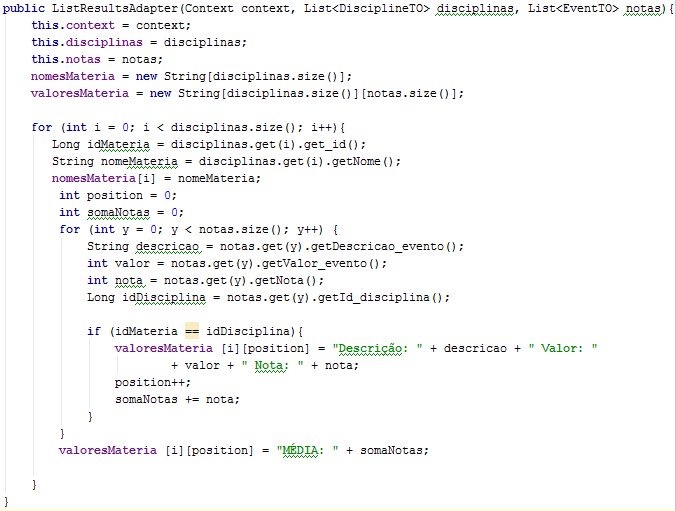
\includegraphics[scale=0.7]{./imagens/2_q_metodologico/4_procedimentos_resultados/42_aplicativo/app8.png}}
		\caption[Adicionando uma dependência ao projeto]{Adicionando uma dependência ao projeto.
		\textbf{Fonte:}Elaborado pelos autores.}
		\label{fig:app9}
	\end{figure}
	
	\par Na tela em que foi aberta localizou-se a biblioteca GSON com o endereço da
Google, logo após selecionou-a e clicou no botão Ok para adicioná-la, como
apresenta a Figura \ref{fig:app10}.
	
	\begin{figure}[h!] 
		\centerline{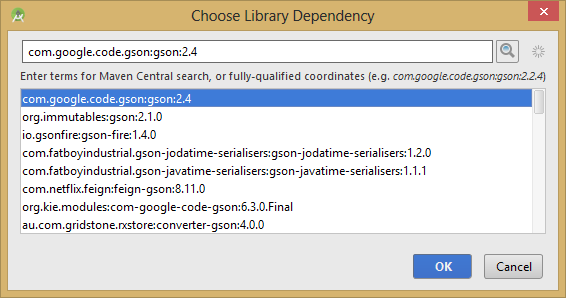
\includegraphics[scale=0.7]{./imagens/2_q_metodologico/4_procedimentos_resultados/42_aplicativo/app9.png}}
		\caption[Adicionando a biblioteca GSON ao projeto]{Adicionando a biblioteca GSON ao projeto.
		\textbf{Fonte:}Elaborado pelos autores.}
		\label{fig:app10}
	\end{figure}
	
	\par Na Figura \ref{fig:app11}, é mostrado o código onde é utilizado a
	biblioteca GSON. O sistema lê os dados vindos em JSON e envia para o GSON que faz a conversão dos
dados no formato da classe \texttt{EventTO}.

	\begin{figure}[h!] 
		\begin{lstlisting}[style=custom_JAVA]
			...
	Reader reader = new InputStreamReader(content);
    Gson gson = new Gson();
    retornoEventos = gson.fromJson(reader, Events.class);
			...
\end{lstlisting}
		\caption[Usando GSON para conversão dos dados]{Usando GSON para conversão dos dados.
		\textbf{Fonte:}Elaborado pelos autores.}
		\label{fig:app11}
	\end{figure}
	
	\par Depois, fez-se necessário construir uma classe que fizesse o gerenciamento
dos dados vindos do banco de dados com a interface que listará as informações
aos usuários. Essa classe recebeu o nome de \texttt{ListResultsAdapter} e
estende da classe nativa do Android denominada
\texttt{BaseExpandableListAdapter}.

	\par Nesta classe foi criado um construtor que recebe a lista de disciplinas
cursadas pelo aluno e uma lista com as notas de cada matéria. Os nomes das
disciplinas foram inseridos em um \textit{array} de \textit{Strings}, já as
notas foram inseridas em uma matriz. Este procedimento foi necessário devido a
estrutura dos métodos \texttt{getGroupView()} e \texttt{getChildView()}
responsável por apresentar na tela do dispositivo os nomes das disciplinas e as
notas das matérias respectivamente.  A Figura \ref{fig:app12} apresenta o
construtor da classe \texttt{ListResultsAdapter}.

	\begin{figure}[h!] 
		\begin{lstlisting}[style=custom_JAVA]
public ListResultsAdapter(Context context, List<DisciplineTO> disciplines, List<EventTO> results){
    this.context = context;
    this.disciplines = disciplines;
    this.results = results;
    namesDisciplines = new String[disciplines.size()];
    EventsDisciplines = new String[disciplines.size()][results.size()];

    for (int i = 0; i < disciplines.size(); i++){
        Long idDiscipline = disciplines.get(i).get_id();
        String nameDiscipline = disciplines.get(i).getName();
        namesDisciplines[i] = nameDiscipline;
        int position = 0;
        int totalResults = 0;
        for (int y = 0; y < results.size(); y++) {
            String description = results.get(y).getDescription_event();
            int value = results.get(y).getValue_event();
            int result = results.get(y).getResult();
            Long disciplineId = results.get(y).getId_discipline();

            if (idDiscipline == disciplineId){
                EventsDisciplines [i][position] = "Descricao: " + description +
                " Valor: " + value + " Nota: " + result;
                position++;
                totalResults += result;
            }
        }
        EventsDisciplines [i][position] = "SOMA DAS NOTAS: " + totalResults;
    }
}
\end{lstlisting}
		\caption[Construtor da classe ListResultsAdapter]{Construtor da classe ListResultsAdapter.
		\textbf{Fonte:}Elaborado pelos autores.}
		\label{fig:app12}
	\end{figure}

	\par Após adicionado os dados no \textit{array} e na matriz é preciso exibí-los
ao estudante. Na Figura \ref{fig:app13}, pode se ver o método \texttt{getGroupView()}
criando um \textit{widget} do tipo \textit{textView}  e inserindo nele o nome
da matéria, os espaçamentos, o tamanho da fonte e informando que as palavras
serão escritos em negrito.

	\begin{figure}[h!] 
		\begin{lstlisting}[style=custom_JAVA]
@Override
    public View getGroupView(int groupPosition, boolean isExpanded,
                             View convertView, ViewGroup parent) {

        TextView textViewDiscipline = new TextView(context);
        textViewDiscipline.setText(namesDisciplines[groupPosition]);
        textViewDiscipline.setPadding(40, 10, 0, 10);
        textViewDiscipline.setTextSize(20);
        textViewDiscipline.setTypeface(null, Typeface.BOLD);

        return textViewDiscipline;
    }
\end{lstlisting}
		\caption[Método getGroupView()]{Método \texttt{getGroupView()}.
		\textbf{Fonte:}Elaborado pelos autores.}
		\label{fig:app13}
	\end{figure}
	
	\pagebreak

	\par O método \texttt{getChildView()} segue a mesma lógica do método
\texttt{getGroupView()}, como ilustra a Fugura \ref{fig:app14}.

	\begin{figure}[h!] 
		\begin{lstlisting}[style=custom_JAVA]
@Override
    public View getChildView(int groupPosition, int childPosition,
                             boolean isLastChild, View convertView, ViewGroup parent) {

        TextView textViewSubList = new TextView(context);
        textViewSubList.setText(EventsDisciplines[groupPosition][childPosition]);
        textViewSubList.setPadding(10, 10, 10, 5);
        textViewSubList.setTextSize(15);

        return textViewSubList;
    }
\end{lstlisting}
		\caption[Método getChildView()]{Método \texttt{getChildView()}.
		\textbf{Fonte:}Elaborado pelos autores.}
		\label{fig:app14}
	\end{figure}
	
	\par O próximo passo, foi criação de uma \textit{activity} do tipo
\textit{blank activity} com finalidade de listar as notas. Ao criá-la com o
nome de \texttt{ListResultsActivity}, o Android Studio gerou dentro da pasta
\textit{layout} o arquivo XML referente a ela, chamado de
\texttt{activity\_list\_results.xml}. Neste, foi inserido apenas o
\textit{widget} \texttt{expandableListView}, que está incumbido de apresentar
a lista de disciplinas cujo o discente está cursando e ao clicar em alguma
dessas matérias serão apresentadas as notas referentes às atividades
realizadas nesta disciplina. Na Figura \ref{fig:app15} é possível ver o código XML de uma
lista do tipo \texttt{expandableListView}.

	\begin{figure}[h!] 
		\begin{lstlisting}[style=custom_XML]
<RelativeLayout 
	xmlns:android="http://schemas.android.com/apk/res/android"
    xmlns:tools="http://schemas.android.com/tools" 
    android:layout_width="match_parent"
    android:layout_height="match_parent" 
    android:paddingLeft="@dimen/activity_horizontal_margin"
    android:paddingRight="@dimen/activity_horizontal_margin"
    android:paddingTop="@dimen/activity_vertical_margin"
    android:paddingBottom="@dimen/activity_vertical_margin"
    android:theme="@style/AppTheme"
    tools:context="univas.edu.com.university.ListResultsActivity">

    <ExpandableListView
        android:layout_width="wrap_content"
        android:layout_height="wrap_content"
        android:id="@+id/expandableListView2"
        android:divider="#FFFFFF"
        android:dividerHeight="1dp"
        android:layout_alignParentBottom="true"
        android:layout_alignParentStart="true"
        android:layout_alignParentTop="true" />

</RelativeLayout>
\end{lstlisting}
		\caption[Código XML do layout que apresentará a lista de notas]{Código XML do
		\textit{layout} que apresentará a lista de notas.
		\textbf{Fonte:}Elaborado pelos autores.}
		\label{fig:app15}
	\end{figure}
	
	\pagebreak
	
	\par Na classe \texttt{ListResultsActivity}, é preciso informar o layout a ser
chamado através do método \texttt{setContentView()}. Também foi necessário
passar para a classe \texttt{ListResultsAdapter} a lista de disciplinas que o
discente está cursando e a lista com as notas referentes a cada matéria vindas
do banco de dados. Na Figura \ref{fig:app16} é exibido o método
\texttt{onCreate()} da classe \texttt{ListResultsActivity}. 
	
	
	\begin{figure}[h!] 
		\begin{lstlisting}[style=custom_JAVA]
@Override
protected void onCreate(Bundle savedInstanceState) {
    super.onCreate(savedInstanceState);
    setContentView(R.layout.activity_list_results);
    helper = new DatabaseHelper(this);

    execute = new DatabaseExecute(helper);

    ExpandableListView listView = 
    		(ExpandableListView) findViewById(R.id.expandableListView2);
    listView.setAdapter(
    	new ListResultsAdapter(
        	this, 
        	execute.getDisciplines(),
        	execute.getResults())
    	); 
}
\end{lstlisting}
		\caption[ Método onCreate() da classe ListResultsActivity]{ Método
		\texttt{onCreate()} da classe \texttt{ListResultsActivity}.
		\textbf{Fonte:}Elaborado pelos autores.}
		\label{fig:app16}
	\end{figure}

	\par Estes procedimentos realizados para as classes
\texttt{ListResultsActivity} e \texttt{ListResultsAdapter} foram necessários
para apresentar as notas dos exercícios resolvidos. Desta mesma forma foi
preciso criar uma \textit{activity} e um \texttt{adapter} tanto para faltas
quanto para provas agendadas seguindo a mesma lógica.

	\par No momento em que algum professor lançar notas, faltas ou provas agendadas
no portal do aluno, é indispensável notificar o estudante. Com esse intuito
desenvolveu-se uma classe chamada de \texttt{GcmIntentServiceUnivas} que
estende \texttt{IntentService}, que recebe a mensagem vinda do GCM.

	\par Esta classe recebe os dados em formato JSON, por isso ela transfere estas
informações para o método \texttt{getJsonEvents()} da classe
\texttt{HttpUtilUnivas}, o qual será responsável por ler os dados e realizar os
procedimentos de gravação no banco de dados.

	\par Ao salvar o evento é chamado o método \texttt{sendNotification()}, que
receberá um objeto da classe \texttt{EventTO}. Ele realiza uma análise do tipo
de evento, para saber qual activity deve ser executada quando o usuário clicar
na notificação. Logo após adicionado os atributos da notificação, como o ícone,
o título e a mensagem, a notificação é exibida ao usuário. Na Figura
\ref{fig:app17} é visível o método \texttt{sendNotification()}.

	\begin{figure}[h!] 
		%\begin{lstlisting}[style=custom_JAVA]
private void sendNotification(EventTO to) {
        String msg;
        DisciplineTO disciplineTO = execute.getDispline(to.getId_discipline());
        String nameDispline = disciplineTO.getName();
        mNotificationManager = (NotificationManager)
                this.getSystemService(Context.NOTIFICATION_SERVICE);
        PendingIntent contentIntent;
        if(to.getType_event().equals("PROVA_AGENDADA")){
            List<String> data = new ArrayList<String>();
            data.add(nameDispline);
            data.add(to.getDescription_event());
            data.add(String.valueOf(to.getValue_event()));
            data.add(to.getDate_event());
            Intent intent = new Intent(this, NotificationAgendasActivity.class);
            intent.putExtra("dados", (ArrayList<String>)data);
            contentIntent = PendingIntent.getActivity(this, 0, intent, 0);

            msg = "Prova agendada dia" + to.getDate_event();
        }else{
            if(to.getType_event().equals("FALTAS")){
                List<String> data = new ArrayList<String>();
                data.add(nameDispline);
                data.add(to.getDate_event());
                data.add(String.valueOf(to.getValue_event()));
                Intent intent = new Intent(this, NotificationFoulsActivity.class);
                intent.putExtra("dados", (ArrayList<String>)data);

                contentIntent = PendingIntent.getActivity(this, 0, intent, 0);

                msg = to.getValue_event() + " falta(s) recebidas";
            }else{
                List<String> data = new ArrayList<String>();
                data.add(nameDispline);
                data.add(to.getDescription_event());
                data.add(String.valueOf(to.getValue_event()));
                data.add(String.valueOf(to.getResult()));
                Intent intent = new Intent(this, NotificationResultsActivity.class);
                intent.putExtra("dados", (ArrayList<String>)data);

                contentIntent = PendingIntent.getActivity(this, 0, intent, 0);
               msg = "Nova nota " + to.getResult();
            }
        }

        Uri soundUri = RingtoneManager.getDefaultUri(RingtoneManager.TYPE_NOTIFICATION);

        NotificationCompat.Builder mBuilder = new NotificationCompat.Builder(this)
        .setSmallIcon(R.drawable.notification_univas)
        .setContentTitle("Univas informa")
        .setAutoCancel(true)
        .setStyle(new NotificationCompat.BigTextStyle()
        .bigText(msg))
        .setContentText(msg)
        .setSound(soundUri);
        
        Vibrator vibrator = (Vibrator) getSystemService(Context.VIBRATOR_SERVICE);
        long milliseconds = 30;
        vibrator.vibrate(milliseconds);

        mBuilder.setContentIntent(contentIntent);
        mNotificationManager.notify(NOTIFICATION_ID, mBuilder.build());
}
\end{lstlisting}
		\caption[Método sendNotification()]{ Método \texttt{sendNotification()}.
		\textbf{Fonte:}Elaborado pelos autores.}
		\label{fig:app17}
	\end{figure}
	

	\par A notificação acontece toda vez que o GCM envia uma informação ao
dispositivo. Para tratar essas ocorrências foi projetada uma classe para ser o
\texttt{BroadcastReceiver} chamada de \texttt{GcmBroadcastReceiverUnivas}. Ela
estende da classe \texttt{WakefulBroadcastReceiver} nativa do Android e possui
apenas um método chamado de \texttt{onReceive()}, o qual receberá a
\textit{intent} a ser chamada quando chegar algum dado do GCM. Na Figura
\ref{fig:app18}, vê-se a classe \texttt{GcmBroadcastReceiverUnivas}, que
através do método \texttt{onReceive()} inicializará a classe
\texttt{GcmIntentServiceUnivas}.

	\begin{figure}[h!] 
		\begin{lstlisting}[style=custom_JAVA]
public class GcmBroadcastReceiverUnivas extends WakefulBroadcastReceiver {

    @Override
    public void onReceive(Context context, Intent intent) {
        ComponentName comp = new ComponentName(context.getPackageName(),  GcmIntentServiceUnivas.class.getName());
        startWakefulService(context, (intent.setComponent(comp)));
        setResultCode(Activity.RESULT_OK);
    }
}
\end{lstlisting}
		\caption[Classe GcmBroadcastReceiverUnivas]{Classe
		\texttt{GcmBroadcastReceiverUnivas}.
		\textbf{Fonte:}Elaborado pelos autores.}
		\label{fig:app18}
	\end{figure}
		
	\par No entanto para configurar esta classe como um \texttt{BroadcastReceiver},
foi preciso adicioná-la na tag \texttt{<receiver>} do arquivo
\texttt{AndroidManifest.XML}, como mostra a Figura \ref{fig:app19}.

	\begin{figure}[h!] 
		\begin{lstlisting}[style=custom_XML]
<receiver
	android:name=".model.GcmBroadcastReceiverUnivas"
	android:permission="com.google.android.c2dm.permission.SEND" >
		<intent-filter>
		    <action android:name="com.google.android.c2dm.intent.RECEIVE" />
		    <category android:name="univas.edu.com.university.model" />
		</intent-filter>
</receiver>
\end{lstlisting}
		\caption[Configuração do BroadcastReceiver no
		AndroidManifest.XML]{Configuração do \texttt{BroadcastReceiver} no
		\texttt{AndroidManifest.XML}.
		\textbf{Fonte:}Elaborado pelos autores.}
		\label{fig:app19}
	\end{figure}

	\par Por fim, foi construída uma classe chamada de \texttt{GcmControllerUnivas}
que tem por objetivo configurar o dispositivo para trabalhar com o GCM.

	\par Nesta classe existe um método denominado \texttt{checkPlayServices()} como
intuito de verificar se o dispositivo possui os requisitos necessários para o
GCM. Na Figura \ref{fig:app20}, é apresentado o método checkPlayServices().

	\begin{figure}[h!] 
		\begin{lstlisting}[style=custom_JAVA]
public boolean checkPlayServices() {

        int resultCode = GooglePlayServicesUtil.isGooglePlayServicesAvailable(context);

        if (resultCode != ConnectionResult.SUCCESS) {

            if (GooglePlayServicesUtil.isUserRecoverableError(resultCode)) {

                GooglePlayServicesUtil.getErrorDialog(
                	resultCode, 
                	new MainActivity(), 
                	PLAY_SERVICES_RESOLUTION_REQUEST
                ).show();

            } else {
                Log.i(TAG, "Este dispositivo nao suporta o GCM.");
            }
            return false;
        }
        return true;
    }
\end{lstlisting}
		\caption[Método checkPlayServices()]{Método \texttt{checkPlayServices()}.
		\textbf{Fonte:}Elaborado pelos autores.}
		\label{fig:app20}
	\end{figure}
	
	\par Logo após é chamado o método \texttt{getRegistrationId()}, que é incumbido
de retornar o \textit{Registration} ID. Na Figura \ref{fig:app21} é possível ver
este método, no entanto, se o registro retornado for nulo, isso significa que o
aparelho não está cadastrado nos servidores da Google, então é executado o
método \texttt{registerInBackground()} que fará esse cadastro, como demostra a
Figura \ref{fig:app22}.

	\begin{figure}[h!] 
		\begin{lstlisting}[style=custom_JAVA]
private String getRegistrationId(Context context) {

        final SharedPreferences prefs = getGcmPreferences(context);

        String registrationId = prefs.getString(PROPERTY_REG_ID, "");
        if (registrationId.isEmpty()) {
            Log.i(TAG, "Falha ao registrar.");
            return "";
        }
  
        int registeredVersion = prefs.getInt(PROPERTY_APP_VERSION, Integer.MIN_VALUE);
        int currentVersion = getAppVersion(context);
        if (registeredVersion != currentVersion) {
            Log.i(TAG, "Versao alterada do aplicativo.");
            return "";
        }
        return ;
}
\end{lstlisting}
		\caption[Método getRegistrationId()]{Método \texttt{getRegistrationId()}.
		\textbf{Fonte:}Elaborado pelos autores.}
		\label{fig:app21}
	\end{figure}
	
	\begin{figure}[h!] 
		\begin{lstlisting}[style=custom_JAVA]
private void registerInBackground() {

        new AsyncTask<Void, Void, String>() {
            @Override
            protected String doInBackground(Void... params) {
                String msg = "";
                try {
                    if (gcm == null) {
                        gcm = GoogleCloudMessaging.getInstance(context);
                    }
                    regid = gcm.register(SENDER_ID);
                    msg = "Dispositivo registrado, registro ID=" + regid;

                    sendRegistrationIdToBackend(regid);

                    storeRegistrationId(context, regid);
                } catch (IOException ex) {
                    msg = "Error :" + ex.getMessage();
                }
                return msg;
            }

            @Override
            protected void onPostExecute(String msg) {
                Toast.makeText(new MainActivity(), msg, Toast.LENGTH_SHORT).show();
            }
        }.execute(null, null, null);
    }
\end{lstlisting}
		\caption[Método registerInBackground()]{Método
		\texttt{registerInBackground()}.
		\textbf{Fonte:}Elaborado pelos autores.}
		\label{fig:app22}
	\end{figure}
	
	\par Desta forma, quando o \textit{web service} envia uma informação ao GCM, o
\textit{Registration} ID é transmitido junto aos dados, gerado pelo método
\texttt{registerInBackground()}, possibilitando ao serviço da Google
identificar a qual dispositivo deve conduzir a mensagem.